% Einleitung
%   - Ziel: Rechtfertigung technischer design entscheidungen, plus überblick über den Code
%   - Creature Generator als Unity Package
%   - Erläutere Aufbau des Kapitels
%       - Der Pipeline folgend, von der Bone Definition, bis zur Creature Generator Klasse
% Settings als ScriptableObjects
%   Creature Parameters
%       - Funktion als zentrales Einstellungsobjekt des Generators
%       - Tabelle mit momentanen Einstellungen
%   Creature Generator Settings
% Bone Definition
%   - Existenzgrund: Generische Datenstruktur für alle möglichen Generatoren
%   - Erläuterung der Datenstruktur
%   - Anatomische Koordinatensysteme
%       - Verweis auf Fachliches Vorgehen für Details
%       - Technischer Grund: Annahmen über Koordinatensysteme werden nicht über Generator grenzen getragen
% Generator Klassen
%   - Instanziieren der Creature Parameters um Knochenlängen an AI zu liefern
%   - Zusammenstecken der Bone Definitions
% Skeleton Definition
%   - 
% Joint Tables und Density Tables
% Skeleton Assembler
%   - Erzeugt Unity Gameobjects aus der Skeleton Definition
% Mesh Generator
\DeclarePairedDelimiter\norm{\lVert}{\rVert}

Im folgenden Kapitel wird zuerst eine organisatorische Übersicht über die Themengebiete des PG649 Creature Generators gegeben, die anschließend im technischen Detail erläutert werden. Ziel des Kapitels ist es zuerst eine Verständnisgrundlage zu schaffen, damit die nachfolgenden technischen Merkmale, Design-Entscheidungen und Kompromisse nachvollziehbar sein werden.

\subsection{Fachliche Umsetzung}

\subsubsection{Parametrische Kreatur}\label{param_method}
Als Grundlage für die parametrische Generierung der Kreaturen dient das von Jon Hudson in seiner Thesis \cite{Hudson2013CreatureGU} beschriebene Modell, welches in Abschnitt \ref{parametrsiche_generatoren} näher beschrieben wird.\\
Die Kreatur besteht aus mehreren Körperteilen, die separat generiert werden und jeweils ihre eigenen Parameter besitzen. Diese Körperteile sind Torso, Beine, Arme, Hals, Füße und Kopf, die jeweils aus einem oder mehreren Knochen bestehen. Alle in diesem Abschnitt erwähnten Zufallsvariablen entstammen einer Kombination aus Gleich- und Normalverteilungen.

\paragraph{Knochen Koordinaten}
Um einfache lokale Transformationen zu ermöglichen, definieren wir ein einheitliches Koordinatensystem für alle Knochen. Der Ursprung dessen ist der \textbf{proximale Punkt}, dieser ist der der Körpermitte am nächsten gelegene Punkt und entspricht somit der Stelle, an der der Knochen, gegebenenfalls mit einem Offset, an seinem Elternknochen befestigt ist. Der \textbf{distale Punkt} ist der Endpunkt des Knochens, also der am weitesten von der Körpermitte entfernte Punkt. \\ Die \textbf{proximale Achse} verläuft parallel zum Knochen, von der Körpermitte weg, also in Richtung des distalen Punktes. Die \textbf{ventrale Achse} liegt orthogonal zur proximalen Achse und zeigt in Richtung der Vorderseite des Knochens. Diese lässt sich prinzipiell beliebig definieren, in unserem Fall haben wir uns jedoch für Armknochen auf die dem Körper zugewandte Innenseite des Knochens festgelegt, für parallel zum Boden generierte Torsi auf die Unterseite und für alle weiteren Knochen auf die der Blickrichtung des Skeletts zugewandten Seite. Die \textbf{laterale Achse} liegt senkrecht auf den beiden zuvor definierten Achsen.

\paragraph{Generierung}
\label{sec:parametricGeneration}
Unsere Methode setzt voraus, dass zunächst gewisse Vorgaben zur generellen Struktur der Kreatur gemacht werden. In unserem konkreten Fall bedeutet dies, dass wir uns zunächst auf Zwei- und Vierbeiner beschränken. Der Zweibeiner orientiert sich an der menschlichen Anatomie und besitzt deshalb in jedem Bein jeweils zwei Knochen und einen einzelnen Fußknochen sowie zwei Arme. Die Beine eines Vierbeiners besitzen, angelehnt an die Skelette echter vierbeiniger Säugetiere, jeweils vier Knochen. Arme werden hier nicht generiert. Um Kreaturen zu erzeugen, die nicht einer dieser Strukturen entsprechen, wie beispielsweise Spinnentiere oder Echsen, müsste man weitere Skelette definieren.\\
\\
Zuerst  wird der \textbf{Torso} Generiert. Im Falle des Zweibeiners ist dieser nach oben gerichten, beim Vierbeiner parallel zum Boden. Als Parameter werden jeweils Minima und Maxima für die Länge und den Umfang des Torsos übergeben. Daraus wird zunächst ein zufälliger Wert für die Länge bestimmt. Da wir uns vorerst für einen Torso bestehend aus drei Knochen entschieden haben, wird diese Länge zufällig auf drei kleinere Längen aufgeteilt. Jeder dieser Knochen erhält dann einen zufälligen Umfang. Das unterste Torsosegment dient als Elternknochen der Kreatur, die anderen beiden Knochen werden dann nacheinander am distalen Punkt des vorangegangenen Knochens befestigt.\\
Anschließend werden die \textbf{Beine} paarweise generiert, wodurch nur symmetrische Kreaturen erstellt werden können. Auch hier wird zunächst die Länge zufällig bestimmt und dann auf zwei beziehungsweise vier Knochen aufgeteilt. Auch die Umfänge werden zufällig bestimmt, jedoch zusätzlich sortiert, sodass das dickste Segment der Körpermitte am nächsten gelegen ist. In beiden Fällen werden die Beine gerade nach unten generiert. Bei einem Zweibeiner wird am distalen Punkt des unteren Beinknochen in Richtung dessen ventraler Achse ein Fußknochen mit parametrisch zufällig bestimmter Größe erzeugt. Befestigt werden die Beine durch einen zusätzlichen Hüftknochen, der parallel zum Torso am proximalen Punkt des ersten Torsoknochens ansetzt und dessen proximale Achse entgegen derer seines Elternknochens gerichtet ist, also den Torso etwas verlängert. Es wird jeweils ein Bein links und rechts vom Mittelpunkt des Hüftknochens angebracht. Der Abstand entlang der lateralen Achse ergibt sich aus dem Umfang des Knochens. Im Falle des Vierbeiners wird analog dazu ein weiteres Beinpaar am distalen Punkt des letzten Torsoknochens generiert. Anschließend werden Torso und Beine so rotiert, dass sich alle Enden der Beine auf der selben Höhe befinden und die Beine noch immer gerade nach unten Zeigen.\\
Die \textbf{Arme} des Zweibeiners werden analog zu den Beinen mit Hilfe eines Schultersegmentes am distalen Punkt des obersten Torsoknochens erzeugt.\\
Der \textbf{Hals} wird als Verlängerung des Torsos generiert. Dabei wird sowohl die Länge und Dicke zufällig bestimmt als auch die Anzahl der Knochen. Beim Zweibeiner wird er am distalen Punkt des Schulterknochens befestigt und alle Knochen zeigen parallel zum Torso gerade nach oben. Beim Vierbeiner erfolgt das Befestigen am distalen Punkt des vorderen Hüftknochens. Dabei ist die Rotation des ersten Knochens ein zufälliger Wert zwischen der proximalen und der negativen ventralen Achse des Elternknochens. Jedes weitere Halssegment erhält eine zufällige Rotation um $\pm 20\degree$.\\
Der \textbf{Kopf} ist ein einzelner Knochen mit zufälliger Länge und Umfang, der als Verlängerung des letzten Halsknochens betrachtet werden kann.\\
\\
Die Glaubwürdigkeit und Variation der Kreaturen ist dadurch also stark von den gewählten Parametern abhängig. Diese werden von Hand gesetzt, wobei größere Wertebereiche auch für größere Unterschiede zwischen den Kreaturen sorgen, aber gleichzeitig die Kontrolle über das Ergebnis einschränken. Die Beschränkungen der Bewegungsradii der Gelenke werden momentan händisch mit erfahrungsgemäß guten Werten gesetzt. Ziel ist es allerdings auch diese in Zukunft soweit möglich prozedural mit Hilfe von Parametern zu erzeugen, um verschiedene Bewegungsmuster zu ermöglichen.




\subsubsection{L-System Kreatur}\label{L_System}
Der erste Ansatz zur Generierung von Kreaturen verwendet ein L-System, um die Struktur des Skelettes zu formalisieren.
Dabei wird jede gezeichnete Strecke der Turtle als ein Knochen interpretiert.
Hierdurch entsteht stets ein zusammenhängendes Skelett, da sich die Turtle nicht fortbewegen kann ohne zu zeichnen.
An Positionen wo die Turtle anhält werden Gelenke (Joints) gelegt.
Mit diesem Ansatz können nicht nur Skelette von Zweibeinern und Vierbeinern erzeugt werden, sondern auch Kreaturen mit beliebig vielen Armen oder Beinen.

\paragraph{Generierung der Skelettstruktur}
Um eine Kreatur mithilfe des L-Systems zu generieren wird zunächst die grundlegende Struktur im Startstring definiert.
Hierbei werden ausgehend von der initialen Richtung der Turtle, Komponenten des Skeletts wie der Kopf, Arme, der Torso und die Beine definiert.
Für jede dieser Körperteile kann ein eigenes Nicht-Terminalsymbol verwendet werden, um das jeweilige Skelett der Komponente zu definieren.
Mit diesem Ansatz kann jedes Körperteil unabhängig von allen anderen entworfen werden.
Mithilfe eines stochastischen L-Systems können diese zudem zufällige Ausprägungen haben.
Beispielsweise ist es einfach, unterschiedlich lange Körperteile zufällig zu generieren.
Allgemein ist es auch möglich eine zufällige Anzahl an Armen und Beinen zu erzeugen, womit direkt sehr unterschiedliche Kreaturen erzeugt werden können, die aber stets die gleiche Grundstruktur haben.
Der Entwurf der einzelnen Körperteile wird durch die Produktionen des L-Systems definiert.

Das Skelett einer Kreatur die durch ein L-System erzeugt wurde, ist in Abbildung~\ref{skeletonlsystemex} dargestellt.
Das L-System, aus dem diese Skelettstruktur entstanden ist, ist im Folgenden gegeben:
\begin{itemize}
	\item Startstring:
	      \begin{equation*}
		      S=\texttt{[}\texttt{|}C\texttt{]}\texttt{+}(90)\texttt{[}AH\texttt{]}\texttt{-}(180)\texttt{[}AH\texttt{]}\texttt{+}(90)T\texttt{+}(90)\texttt{[}G\texttt{-}(90)L\texttt{]}\texttt{-}(180)\texttt{[}G\texttt{+}(90)L\texttt{]}
	      \end{equation*}
	\item Iterationen: 2
	\item Produktionen:
	      \begin{align*}
		      A\rightarrow & ~F(0.25)F(0.25)                          & \text{Arme}  \\
		      L\rightarrow & ~F(0.35)F(0.3)\texttt{\textasciicircum}V & \text{Beine} \\
		      T\rightarrow & ~F(0.4)F(0.4)                            & \text{Torso} \\
		      C\rightarrow & ~F(0.3)                                  & \text{Kopf}  \\
		      G\rightarrow & ~F(0.2)                                  & \text{Hüfte} \\
		      V\rightarrow & ~F(0.2)                                  & \text{Füße}  \\
		      H\rightarrow & ~F(0.15)                                 & \text{Hände}
	      \end{align*}
\end{itemize}

Die Werte in den Klammern hinter einigen Symbolen sind Argumente für die Fortbewegung und Drehung der Turtle.
Bei dem Auswerten eines $F$ bewegt sich die Turtle normalerweise um eine Einheit in die aktuelle Richtung.
Der Wert in den Klammern hinter dem $F$ überschreibt dies, sodass bspw. $F(0.2)$ die Turtle nur um $0.2$ Einheiten fortbewegen lässt.
Ähnlich ist dies bei den Terminalsymbolen \texttt{+} und \texttt{-}, wo das Argument den Grad $\delta$ angibt, um wie viel sich die Turtle in der Ebene drehen soll.

\begin{figure}[h]
	\begin{center}
		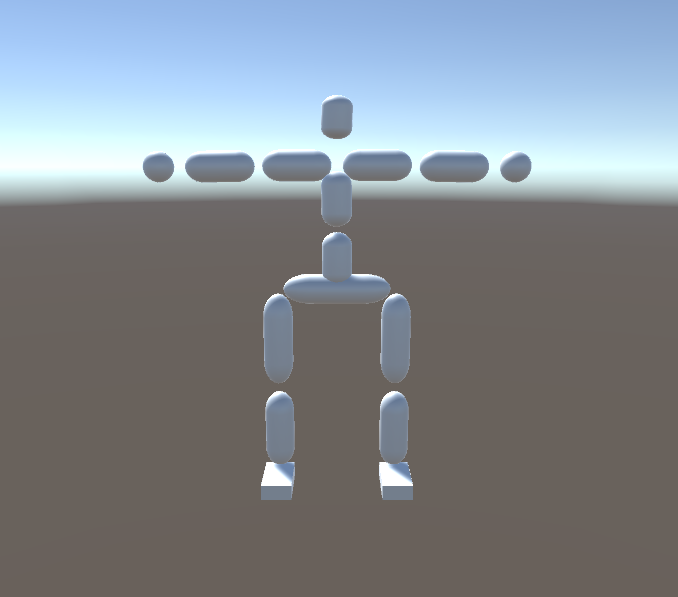
\includegraphics[width = 0.5\textwidth]{resources/img/skeletonlsystemex.png}
	\end{center}
	\caption[L-System Kreatur]{Mittels L-System generiertes Skelett}
	\label{skeletonlsystemex}
\end{figure}

Der resultierende String des L-Systems wird von der Turtle von links nach rechts, den Regeln entsprechend, durchlaufen.
Die Turtle bewegt sich dabei im dreidimensionalen Raum, wie in Abschnitt~\ref{subsub: L-System 3D} beschrieben.
Für jede Fortbewegung der Turtle wird jeweils ihre Startposition und die Endposition im dreidimensionalen Raum als ein Tupel gespeichert.
Die Tupel können als Strecken interpretiert werden, die daraufhin als Knochen dargestellt werden.
Am Ende bildet die Liste der Tupel von Start- und Endpunkten die Skelettstruktur.
Um die Joints sinnvoll definieren zu können, muss festgehalten werden welche Produktion das jeweilige Tupel erzeugt hat.
Dies ist notwendig, da die Produktionen die Kategorien der Körperteile definieren und die Joints dementsprechend angepasst generiert werden müssen.
Ausgehend von dieser Liste werden die Knochen erstellt und mit den Joints zu einem vollständigen Skelett zusammengesetzt.

\paragraph*{Skelett aus L-System generieren}\label{sec:lsystemskel}
Ausgehend von einer Liste von Tupeln, die jeweils Start und Endpunkte einer von der Turtle gezeichneten Strecke enthalten wird das Skelett mit Unity Klassen generiert. Zunächst wird die Liste in eine Baumstruktur überführt. Dabei entspricht ein Knoten im Baum einem Knochen im Skelett. Zwei Knoten stehen in einer Eltern-Kind-Beziehung im Baum, wenn die zugehörigen Strecken sich schneiden. Dabei wird gefordert, dass der Endpunkt der zum Elternknoten gehörigen Strecke dem Startpunkt der zum Kindknoten gehörigen Strecke gleicht. Da angenommen wird, dass es zu jedem Startpunkt eines Tupels in der Liste ein weiteres Tupel gibt, dessen Endpunkt dem Startpunkt gleicht, lässt sich der Baum so definieren. Der Baum wird traversiert und zu jedem Knoten wird ein GameObject erstellt.  Dieses wird mit einem Rigidbody, einem CapsuleCollider und einem primitiven Mesh versehen. Die Knochen werden in Kategorien, wie zum Beispiel Arm, Bein oder Kopf eingeteilt. Zwei Knochen werden mit einem Joint verbunden, wenn sie im Baum in einer Eltern-Kind-Beziehung stehen. Für die erlaubten Rotationen der Joints wurden Standardwerte je nach Kategorie festgelegt. Abbildung \ref{skeletonlsystemex} zeigt ein über ein L-System generiertes Skelett.



\subsubsection{Mesh-Generierung}
\paragraph{Metaball}\label{Metaball_Gen}
Zur Generierung der Geometrie der Kreatur verwenden wir, angelehnt an den Ansatz von Madis Janno \cite{Janno20182dCG} (siehe Abschnitt \ref{sec:metaball}), eine modifizierte Form von Metaballs. Dabei werden genau so viele Bälle entlang eines Generierten Segments platziert wie benötigt werden um zu garantierten, dass dadurch in jedem Fall ein zusammenhängendes Mesh entsteht. Tatsächlich ist jedoch der Einfluss nahegelegener Kugeln aufeinander so groß, dass dadurch nicht nur die minimale Berührung der einzelnen Kugeln entsteht, sondern diese glatt ineinander übergehen. Wie auch bei Janno lässt sich unsere Methode mit beliebigen Metaball-Funktionen durchführen. Aufgrund der guten Ergebnisse haben wir uns jedoch vorerst auf die gleiche, zuerst von Ken Perlin beschriebene, Falloff-Funktion festgelegt:
\[f_i(\vec{x}) = exp(B_i - \frac{B_ir_i^2(\vec(x))}{R_i^2}).\]
Für Metaball $i$ ist $R_i$ dessen Radius, $B_i$ ein Parameter zur Einstellung der "Blobbiness", welcher beeinflusst wie sehr sich Metaballs miteinander verbinden. Wir verwenden den Wert $B_i = 0.5$. $r_i(\vec{x})$ ist der Abstand des Punktes $\vec{x}$ zum Zentrum $c_i$ von Metaball $i$, also: \[r_i(\vec{x})=||\vec{x}-\vec{c_i}||=\sqrt{(x_x-c_{ix})^2+(x_y-c_{iy})^2+(x_z-c_{iz})^2}.\]

Die generierten Kreaturen bestehen aus mehreren Segmenten (Knochen) mit jeweils einem Start- und Endpunkt sowie einer Dicke, die als Radius der darauf platzierten Metaballs verwendet werden kann. Entlang dieser Segmente soll dann das Mesh erzeugt werden. Die von Janno beschriebene Methode berechnet dafür, abhängig von der gewählten Falloff-Funktion, die minimale Anzahl an Metabällen für ein Segment und platziert diese gleichmäßig entlang dessen. Das Problem, welches sich daraus bei unseren Experimenten ergeben hat, liegt darin, dass mit höherer Komplexität der Kreaturen und einer damit einhergehenden steigenden Anzahl an Segmenten, der Einfluss von benachbarten Segmenten nicht gut kontrollieren lässt und diese teilweise ineinander verschmelzen. \\

Unser Ansatz um dieses Problem zu umgehen ist es, die Anzahl der einzelnen Metabälle drastisch zu reduzieren. Anstatt einer beliebig großen Zahl an Bällen entlang jedes Segments, erzeugen wir jeweils nur einen einzigen Körper. Dazu ersetzen wir die Bälle durch Kapseln, also Zylinder mit jeweils durch eine Halbkugel abgerundeten Enden, weshalb wir diese auch als \glqq{Metakapseln}\grqq{} bezeichnen. Möglich macht uns dies eine Modifikation der Falloff-Funktion, beziehungsweise der darin verwendeten Distanz. Wir berechnen hierbei nicht den Abstand zum Zentrum einer Kugel, sondern zu der Verbindungslinie zwischen Start- und Endpunkt. \\

\begin{figure}[ht]
	\centering
	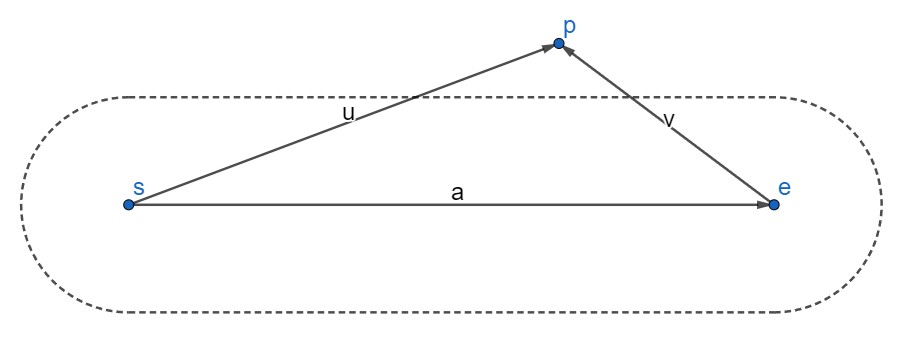
\includegraphics[width=0.7\textwidth]{resources/img/metacapsule.png}
	\caption{Beispiel Metakapsel; Die gestrichelte Linie enthält alle Punkte mit $r=R$}
	\label{metacapsule}
\end{figure}

Um diese Form zu erzeugen muss lediglich die Funktion $r(\vec{x})$ zur Berechnung des Abstandes angepasst werden.
Sei $s$ der Startpunkt, $e$ der Endpunkt, $a$ der Vektor $e-s$, $p$ ein Punkt, dessen Abstand berechnet werden soll, $u=p-s$ und $v=p-e$ (Siehe Abbildung \ref{metacapsule}). Die Distanz lässt sich dann folgendermaßen bestimmen:
\[
	r(\vec{x})=
	\begin{cases}
		||p-s||,                            & \text{falls } a\cdot u < 0 \\
		||p-e||,                            & \text{falls } a\cdot v > 0 \\
		\norm*{\frac{a\times u}{\norm{a}}}, & \text{sonst}.
	\end{cases}
\]

Es werden drei Fälle unterschieden. Liegt der Punkt $p$ im Falle von Abbildung \ref{metacapsule} links von $s$, beziehungsweise rechts von $e$, ist Die Distanz von $p$ zum Segment einfach der euklidische Abstand zum jeweiligen Punkt. Ob dies der Fall ist, lässt sich mit Hilfe der Skalarprodukte $a\cdot u$ beziehungsweise $a\cdot v$ überprüfen. Ansonsten berechnet man die Distanz von Punkt p zur Geraden, die durch $s$ und $e$ verläuft.\\

Da dies nur eine Erweiterung der Metaball-Funktion ist, lassen sich diese Kapseln weiterhin mit anderen Metabällen kombinieren. So können auch Körperteile erstellt werden, die nicht aus solchen Segmenten bestehen, oder Details aus kleineren Metabällen entland der Segmente platziert werden. Grundsätzlich lassen sich auf diese Weise beliebig geformte Objekte, die mit einer solchen Funktion definiert werden, einbinden.
Da die Kapsel nur zylindrisch geformte Segmente darstellen lässt, die in alle Richtungen den gleichen Radius besitzen, haben wir eine weitere Modifikation vorgenommen, die es erlaubt die Metakapsel entlang der ventralen oder lateralen Achse zu strecken beziehungsweise zu stauchen. Dadurch ist es uns möglich Körperteile mit unterschiedlichen Abmessungen entlang der verschiedenen Achsen darzustellen und dennoch unnatürlich wirkende Formen wie beispielsweise einen Quader zu vermeiden.
Dazu bestimmen wir bei der Berechnung von $r(\vec{x})$ zunächst den Vektor, der die kürzeste Verbindung von $\vec{x}$ und dem Segment darstellt, anstatt direkt dessen Länge auszuwerten. Diesen Vektor skalieren wir anschließend entlang der gewünschten Achse. Die Länge des skalierten Vektors ist dann die neue Distanz.

\paragraph{Mesh Indexing}
Zur weiteren Verarbeitung des Meshes beim automatischen Rigging, ist es wichtig, dass das Mesh korrekt indiziert ist, sodass keine doppelten Vertices existieren. Außerdem können so die ausgehenden Kanten der Vertices bestimmt werden, welche ebenfalls später für das automatische Rigging benötigt werden. Während des Marching-Cubes Algorithmus werden die entstehende Dreiecke in eine gesonderte Datenstruktur hinzugefügt, welche für jeden Vertex prüft, ob dieser bereits im Vertex-Buffer existiert. Falls ja, wird kein neuer Vertex eingefügt, sondern das Dreieck referenziert den Vertex über den Index-Buffer. Neue Vertices werden dem Vertex-Buffer hinzugefügt und das entsprechende Dreieck referenziert den neuen Vertex. Die Anzahl der Vertices wird dadurch außerdem signifikant verringert, was Performance-Vorteile beim Rendering und bei der Weiterverarbeitung des Meshes ermöglicht.

\paragraph{Delaunay Triangulation}
In der Entwicklung des automatischen Riggings des Modells wurde festgestellt, dass die Triangulierung des Meshes, welches durch Marching Cubes entsteht nicht numerisch stabil genug ist, um mit der Bone-Heat Methode die Vertex-Gewichte zu berechnen. Für die Lösung des Matrix-Systems der Bone-Heat Methode ist es wichtig, dass die Triangulierung die Delaunay-Bedingung erfüllt~\cite{laplace_beltrami_paper}.

Eine Delaunay-Triangulierung maximiert das Minimum von allen Winkeln in der Triangulierung~\cite{delaunay}. Diese Triangulierung vermeidet Dreiecke die extrem lang und dünn sind. Eine Triangulierung erfüllt die Delaunay-Bedingung genau dann, wenn der Umkreis jedes Dreiecks leer ist. Der Umkreis eines Dreiecks ist der Kreis, der alle Ecken des Dreiecks schneidet.

Die Triangulierung, die bereits durch den Marching Cubes Algorithmus entstanden ist, kann durch die \glqq{Edge-Flipping}\grqq{} Technik in eine Delaunay Triangulierung transformiert werden~\cite{delaunay}. Dazu iteriert der Algorithmus durch alle Kanten des Meshes und prüft für die beiden anliegenden Dreiecke der Kante, ob die gegenüberliegenden Winkel $\alpha$ und $\beta$ kleiner oder gleich $180\degree$ sind. Die Bedingung $\alpha+\beta \leq 180\degree$ ist equivalent zu der Delaunay-Bedingung der beiden Dreicke. Wenn die Delaunay-Bedingung nicht erfüllt ist, können die Dreiecke durch eine \glqq{flip}\grqq{} Operation korrigiert werden. Dabei wird die gemeinsame Kante $BD$ der Dreiecke $\triangle ABD$ and $\triangle BCD$ in eine Kante $AC$ mit Dreiecken $\triangle ABC$ and $\triangle ACD$ geändert. Für das gesamte Mesh kann so lange die `flip' Operation ausgeführt werden, bis alle Dreiecke delaunay sind.

Die \glqq{edge-flip}\grqq{} Operation ist auf der Mesh-Datenstruktur, welche in 3D-Engines wie Unity verwendet wird, relativ aufwendig, da diese keine Möglichkeit bietet, die zugehörigen Dreiecke einer Kante zu finden. In diesem Projekt wurde daher die Polygon Mesh Processing Bibliothek (PMP)~\cite{pmp-library} verwendet. Diese enthält bereits viele Methoden um 3D-Meshes auf komplexe Weise zu modifizieren. Insbesondere wird eine optimierte Datenstruktur für das Mesh genutzt, welche es erlaubt schnell über alle Kanten zu iterieren und diese ohne großen Aufwand zu flippen.

\subsubsection{Automatisches Rigging}
Um die Knochen-Struktur des generierten Skelettes mit dem Mesh zu verknüpfen, muss bei der 3D-Modellierung der Prozess des Riggings durchlaufen werden. Dieser beschreibt wie sich jeder einzelne Vertex des Meshes mit den Knochen in der Szene bewegt. Jeder Vertex kann an beliebig vielen Knochen angehängt werden. Durch eine Gewichtung wird bestimmt wie sehr ein Vertex durch der Transformation eines Knochens mitbewegt wird.
Da sowohl das Skelett, als auch das gesamte Mesh prozedural generiert werden, kann das Rigging nicht wie üblich in einem Modellierungs-Tool wie Blender~\cite{blender} manuell durchgeführt werden, sondern muss zur Laufzeit des Spiels während der Generierung der Kreaturen geschehen.

Für ein erfolgreiches Rigging ist es wichtig, dass das Skelett bereits sinnvoll in dem Mesh eingebettet ist. Da hier das Mesh aus Metaballs generiert wird, welche um die Knochen plaziert sind, können wir hier davon ausgehen, dass das Mesh das Skelett bereits \glqq{sinnvoll}\grqq{} umhüllt.


\begin{figure}[h!]
	\centering
	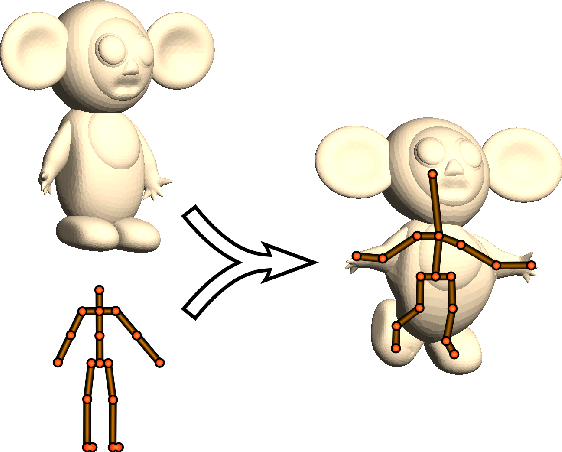
\includegraphics[width=0.6\linewidth]{resources/img/skeleton_embedding.png}
	\caption{Beispiel für ein korrekt eingebettetes Skelett in einem Mesh~\cite{bone_heat_paper}.}
	\label{fig:skeleton_embedding}
\end{figure}

Während der Entwickelung wurde zunächst eine triviale Methode als Zwischenlösung verwendet. Dabei wurden alle Vertices nur an den Knochen mit der geringsten Distanz angehängt. Diese Methode ist jedoch visuell nicht brauchbar, da bei Bewegung des Skeletts an den Gelenken zwischen den Knochen Löcher und verschiedene andere Artefakte entstehen. Es wird also eine Lösung benötigt die es ermöglicht Vertices an mehrere Knochen anzuhängen und die Gewichte so bestimmt, dass das Mesh an den Übergängen zwischen den Knochen möglichst natürlich deformiert wird.

\paragraph{Bone-Heat Methode}
Ein bereits bekannter Algorithmus zur automatischen Gewichtsberechnung und Verknüpfung des Meshes ist die Bone-Heat Methode~\cite{bone_heat_paper}. Dieser berücksichtig mehrere zusätzliche Eigenschaften für die Gewichte. Zuerst sollen die Gewichte unabhängig von der Auflösung des Meshes sein. Außerdem müssen die Gewichte sich sanft über den Verlauf der Oberfläche verändern. Die Breite des Übergangs zwischen zwei Knochen sollte ungefähr proportional zu der Distanz des Gelenks zur Oberfläche des Meshes sein.
Ein Algorithmus, welcher die Gewichte alleine aus der Distanz der Knochen zu den Vertices berechnet, kann oft schlechte Ergebnisse liefern, da er die Geometrie des Modells ignoriert. Zum Beispiel können Teile des Torsos mit einem Arm verbunden werden. Die Bone-Heat Methode behandelt stattdessen das innere Volumen des Modells als einen wärmeleitenden Körper. Es werden für jeden Vertex die Gleichgewichts-Temperatur berechnet und diese als Gewichte für die Knochen verwendet. Wie in Abbildung~\ref{fig:bone_heat_equilibrium} zu sehen ist, wird ein Knochen auf 1° gesetzt und der andere auf 0°. Bei Deformation der beiden Knochen mit den Gewichten aus dem Temperatur-Gleichgewichts entsteht an dem Gelenk eine natürlich aussehende Verformung der Oberfläche.

\begin{figure}[h!]
	\centering
	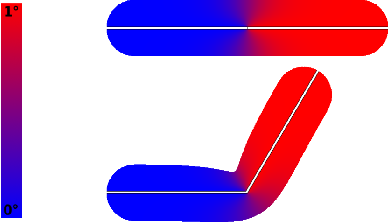
\includegraphics[width=0.7\linewidth]{resources/img/bone_heat_equilibrium.png}
	\caption{Temperatur-Gleichgewicht für zwei Knochen~\cite{bone_heat_paper}.}
	\label{fig:bone_heat_equilibrium}
\end{figure}

Das Temperatur-Gleichgewicht des Volumens zu berechnen wäre sehr aufwändig und langsam, deswegen wird das Gleichgewicht nur über die Oberfläche des Meshes berechnet~\cite[S.~6]{bone_heat_paper}. Die Gewichte für Knochen $i$ werden berechnet durch:

\begin{equation}
	\label{eq:bone_heat}
	\begin{aligned}
		     & \frac{\partial\mathbf{w}^i}{\partial t} = \Delta\mathbf{w}^i+\mathbf{H}\left(\mathbf{p}^i-\mathbf{w}^i\right)=0 \\
		\iff & -\Delta\mathbf{w}^i+\mathbf{H}\mathbf{w}^i=\mathbf{H}\mathbf{p}^i                                               \\
		\iff & \left(-\Delta+\mathbf{H}\right)\mathbf{w}^i=\mathbf{H}\mathbf{p}^i.
	\end{aligned}
\end{equation}

Dabei ist $\Delta$ der diskrete Laplace-Beltrami Operator auf der Oberfläche des Meshes, welcher mit der Kotangens-Methode approximiert wird~\cite{laplace_beltrami_paper}. $\mathbf{p}^i$ ist ein Vektor mit $p^i_j=1$ wenn der nächste Knochen zum Vertex $j$ der Knochen $i$ ist. Sonst ist $p^i_j=0$. $\mathbf{H}$ ist eine Diagonalmatrix in der $H_{jj}$ die Hitze des nächstgelegenen Knochen von Vertex $j$ ist. Sei $d(j)$ die Distanz zum nächstgelegenen  Knochen von Vertex $j$, dann wird $H_{jj}=c/d(j)^2$ gesetzt. Allerdings nur wenn das Geradensegment von dem Vertex zu dem Knochen vollständig in dem Volumen des Modells enthalten ist. Wenn der Knochen von dem Vertex aus also nicht sichtbar ist, wird $H_{jj}=0$ gesetzt. Dies verhindert, dass beispielsweise Vertices des Arms an den Torso angehängt werden. Wenn mehrere Knochen nahezu die gleiche Distanz zu dem Vertex haben und sichtbar sind, werden ihre Anteile an der Temperaturverteilung gleich berücksichtigt. $p_j$ wird dann $1/k$ und $H_{jj} = kc/d(j)^2$.

Der benötigte Sichtbarkeits-Test für die Vertices wurde in diesem Projekt durch ein Signed-Distance-Field (SDF) realisiert, welches wir vorab mit einem Geometry-Shader generieren~\cite{signed_distance_field}. Damit werden effiziente Raycast-Operationen in dem Mesh möglich.
Der Parameter $c$ wird in dem Paper~\cite{bone_heat_paper} auf $1$ gesetzt, um natürlichere Ergebnisse zu erreichen. Für $c\approx0.22$ würde der Algorithmus Gewichte berechnen die ähnlicher zu dem Temperatur-Gleichgewicht über dem tatsächlichen Volumen des Meshes sind.

\paragraph{Lösen des Laplace-Beltrami Systems}
Für die effiziente Lösung des Matrix-Systems in Formel \ref{eq:bone_heat} ist es wichtig die Eigenschaften des diskreten Laplace-Beltrami Operators $\Delta$ näher zu betrachten. Der Operator wird durch die Kotangens-Methode approximiert, indem von jedem Vertex $x_i$ für jede ausgehende Kante ein Gewicht $v(x_i,x_j)$ aus den gegenüberliegenden Winkel $\alpha_{ij}$ und $\alpha_{ji}$ berechnet wird (siehe Abbildung~\ref{fig:cotangent_approx}).

\begin{figure}[h!]
	\centering
	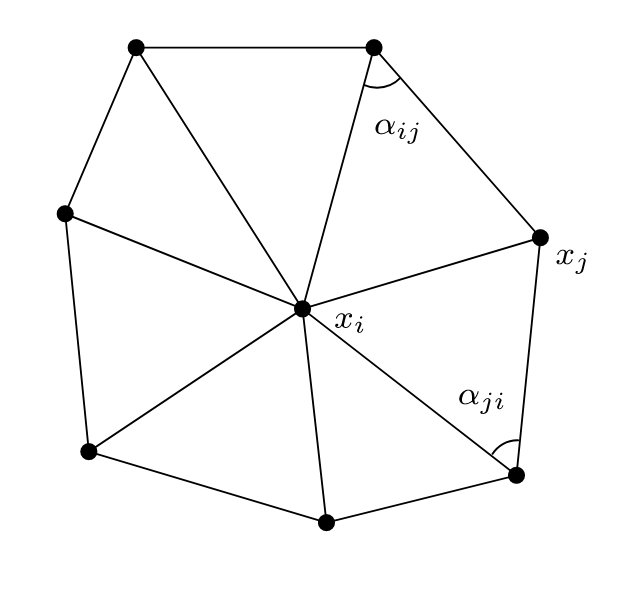
\includegraphics[width=0.4\linewidth]{resources/img/cotangent_approx.png}
	\caption{Berechnung der $\alpha$-Winkel für eine innere Kante~\cite{laplace_beltrami_paper}.}
	\label{fig:cotangent_approx}
\end{figure}

\begin{equation}
	\label{eq:cotangent_weight}
	v(x_i,x_j) =
	\begin{cases}
		\cot{\alpha_{ij}}+\cot{\alpha_{ji}}\  & \text{für innere Kanten} \\
		\cot{\alpha_{ij}}                     & \text{für äußere Kanten}
	\end{cases}
\end{equation}

Aus den Kotangens-Gewichten aus Gleichung~\ref{eq:cotangent_weight} kann nun in Formel~\ref{eq:laplace_beltrami} der Laplace-Beltrami Operator in seiner Matrix-Form berechnet werden \cite{spd_solver_paper,laplace_beltrami_paper}. Dabei bescheibt $N(x_i)$ die Menge der benachbarten Vertices von $x_i$. Da für das Lösen der Gleichung~\ref{eq:bone_heat} lediglich die Matrix $(-\Delta+\textbf{H})$ benötigt wird, kann diese in der Implementierung direkt als eine Matrix erstellt werden. Die Normalisierungsfaktoren aus~\cite{spd_solver_paper} entfallen für diese Anwendung.

\begin{equation}
	\label{eq:laplace_beltrami}
	\Delta_{ij}=
	\begin{cases}
		0                                & i \neq j, x_j \notin N(x_i) \\
		v(x_i,x_j)                       & i \neq j, x_j \in N(x_i)    \\
		-\sum_{x_j\in N(v_i)} v(x_i,x_j) & i = j                       \\
	\end{cases}
\end{equation}

Da die Matrix $\textbf{H}$ eine Diagonalmatrix ist und der Operator $\Delta$ eines Vertex durch seine direkten Nachbarn lokal definiert ist, ist die zu lösende Matrix extrem dünn besetzt. Durch die Euler-Charakteristik für Dreiecks-Netze ergeben sich nur ungefähr $7$ Einträge pro Reihe in der Matrix~\cite{spd_solver_paper}. Ein solches System lässt sich, wie in~\cite{spd_solver_paper} gezeigt, sehr effizient lösen, wenn es sich um eine SPD-Matrix (symmetrisch positiv definit) handelt. Die Matrix ist durch die Konstruktion in Gleichung~\ref{eq:laplace_beltrami} symmetrisch. Für die Lösung dieses Systems wurde in diesem Projekt die Bibliothek Eigen~\cite{eigen} verwendet, welche zahlreiche Methoden zur Matrix-Berechnung bereitstellt. Es wurde der Matrix-Solver \texttt{SparseLU} verwendet, welcher auf dünn besetzte SPD-Matrizen spezialisiert ist.

Durch die Lösung des Systems für jeden Knochen $i$ erhalten wir einen Vektor $\textbf{w}^i$ aus Gleichung~\ref{eq:bone_heat}. Wir hängen jeden Vertex mit dem entsprechenden Gewicht an diesen Knochen, falls das Gewicht größer als $0$ ist. Für die Verwendung der Gewichte in Unity mussten diese außerdem pro Vertex absteigend sortiert und normalisiert werden, sodass sie sich zu $1$ aufsummieren.

\subsubsection{Skinning}\label{skinning}
Nachdem das Mesh durch den Prozess des Riggings mit den Vertex-Gewichten an das Skelett angehängt wurde, muss noch definiert werden, wie das Mesh die Transformationen des Skeletts umsetzt. Für diesen Prozess des \glqq{Skinnings}\grqq{} existieren im allgemeinen zwei unterschiedliche Ansätze.

Die einfachere Technik ist das Linear Blend Skinning (LBS). Hier werden die Vertices wie in Formel~\ref{eq:lbs_skinning} transformiert. Der Vertex $\textbf{v}$ wird zunächst mit allen Knochen-Transformationen $\textbf{C}^j$ transformiert und dann wird der gewichtete Durchschnitt mit den entsprechenden Vertex-Gewichten $w^j$ verwendet um $\textbf{v$'$}$ zu bestimmen.
\begin{equation}
	\label{eq:lbs_skinning}
	\textbf{v$'$} = \sum_{j=0}^n w^{j} \textbf{C}^j \textbf{v}
\end{equation}
LBS hat allerdings den Nachteil, dass einige Transformationen an den Gelenken unnatürlich \glqq{aufrollen}\grqq{}. Dieser sogenannte \glqq{Candy-Wrapper}\grqq{} Effekt ist in Abbildung~\ref{fig:dqs} (links) zu erkennen.

Um dieses Problem zu beheben kann alternativ die Dual Quaternion Technik verwendet werden. Hier wird anstatt einer Linear-Kombination über die transformierten Vertices eine Linear-Kombination über duale Quaternionen berechnet~\cite{dqs}. Diese erlauben es bei der Transformation der Vertices die Skalierung des Mesh-Volumens beizubehalten, da duale Quaternionen sowohl Rotation, als auch Verschiebung gleichzeitig kodieren. Die Implementierung des DQ-Skinnings ist mit kleinen Anpassungen aus dem Projekt~\cite{dqs_github} entstanden. In Abbildung~\ref{fig:dqs} kann man auf der rechten Seite erkennen, das DQS die Probleme von LBS erfolgreich verhindert.

\begin{figure}[h!]
	\centering
	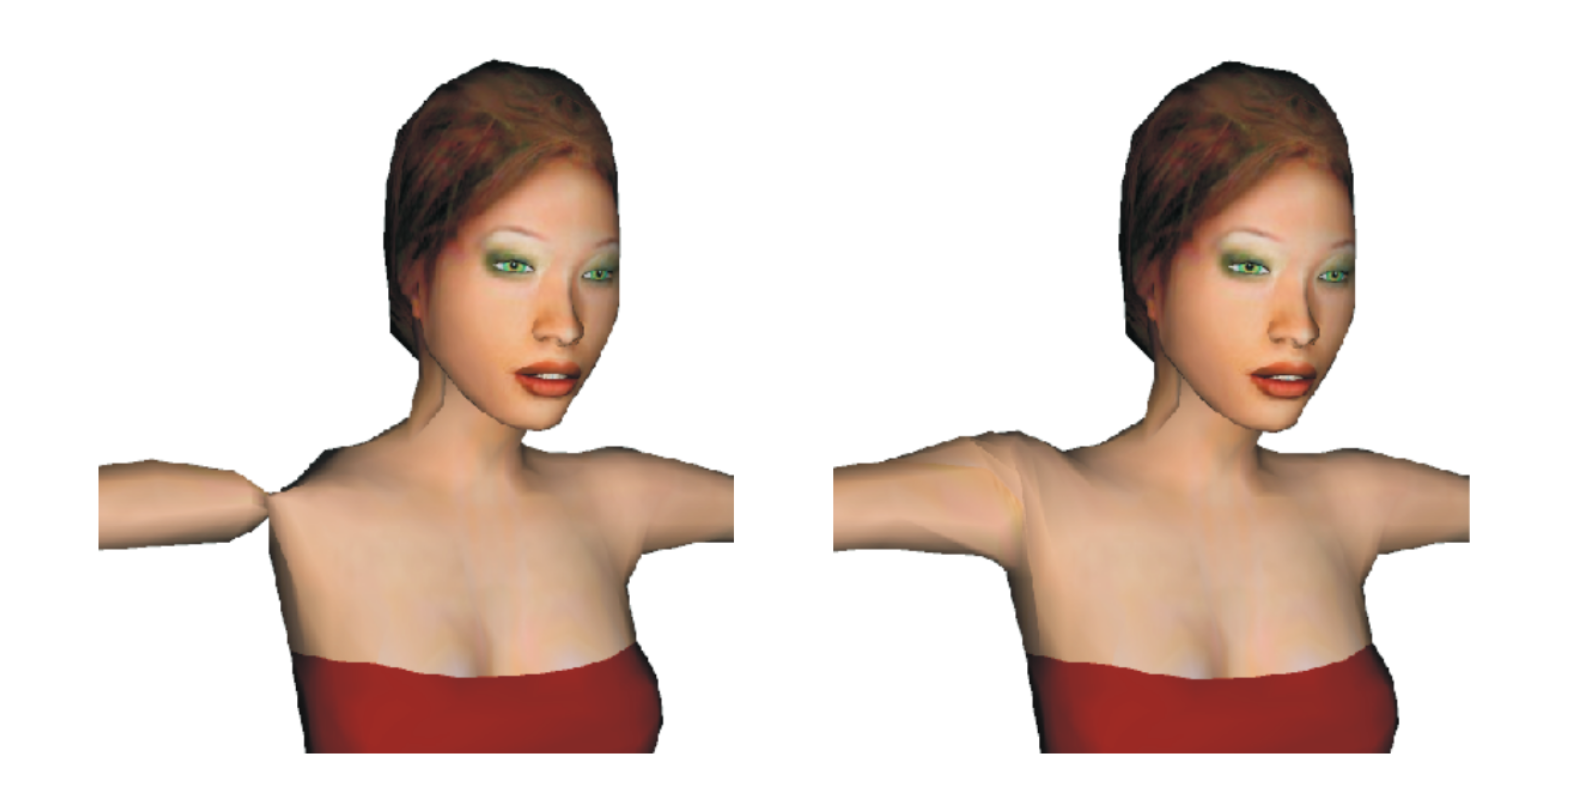
\includegraphics[width=0.7\linewidth]{resources/img/dqs.png}
	\caption{Vergleich von Linear Blend Skinning (links) und Dual Quaternion Skinning (rechts)~\cite{dqs}.}
	\label{fig:dqs}
\end{figure}




%-------------------------------------------------------------------------------------------------------------


\subsection{Technische Umsetzung}

\subsubsection{Unity Package}
Der Generator wird als unabhängiges Unity Package entwickelt.
So kann der Generator einfach in KI-Lernumgebungen und das spätere Spiel eingebunden werden und es wird eine saubere API für den Generator ermutigt.

Die Dateistruktur des Generators unterscheidet sich damit von einem typischen Unity Projekt. Statt im \texttt{Assets}-Ordner, liegen alle hier erläuterten Klassen in \linebreak\texttt{Packages/com.pg649.creaturegenerator/Runtime}.
Der \texttt{Assets}-Ordner enthält lediglich Debug-Skripte, die nicht exportiert werden sollen.

\subsubsection{Konfiguration}
Die Klassen \texttt{Creature\-Generator\-Settings} und \texttt{Parametric\-Creature\-Settings} enthalten alle Konfigurationsmöglichkeiten für den Generator.
Sie sind der Hauptweg mit dem Nutzer mit dem Generator interagieren und bilden somit den Anfang der Tour.

Die Klasse \texttt{CreatureGeneratorSettings} enthält Einstellungen, die das Verhalten des Generators und der generierten Kreaturen bestimmen.
Dazu gehören Einstellungen die zum Beispiel das generieren eines Meshes für die Kreatur abschalten, Einstellungen für das physikalische Verhalten der Kreature, sowie Einstellungen für Debug-Optionen.
Die individuellen Einstellungen sind in der Klasse selbst dokumentiert und werden hier nicht einzeln aufgeführt.

Die Klasse \texttt{ParametricCreatureSettings} enthält Einstellungen, die das Aussehen der generierten Kreaturen bestimmen.
Die Einstellungen definieren Intervalle für die erlaubte Länge, Dicke, und ggbf. Anzahl für Knochen bestimmter Kategorien.
Wieder sind die individuellen Einstellungen in der Klasse selbst dokumentiert.

Beide Konfigurationsklassen sind sogenannte \texttt{ScriptableObjects}.
Sie können von Unity serialisiert und als Assets gespeichert werden.
So können für das spätere Spiel Einstellungen für verschiedene Kreaturen genau so mit exportiert werden wie beispielsweise Shader.
Außerdem ist es möglich die Einstellungen mittels \texttt{git} zu versionieren.

\subsubsection{Bone Definition}
Eine der ersten Datenstrukturen, die von dem Generator erzeugt werden, ist ein Baum von \texttt{BoneDefinition}s.
Dieser Baum bildet die abstrakteste Darstellung eines Skeletts und dient als generisches Ziel für die Generatoren der verschiedenen Kreaturen-Typen.
Jede \texttt{BoneDefinition} enthält die Details eines Knochens, d.h. um was für einen Knochen es sich handelt (Arm, Bein, etc.), die Länge und Dicke des Knochens, die Ausrichtung seines lokalen Koordinatensystems, und Informationen dazu, wie der Knochen für das finale Skelett an seinem Eltern-Knochen angebracht werden soll.

Letztere Informationen werden \texttt{AttachmentHint} genannt und erlauben es Knochen relativ zur Größe des Elternknochens zu positionieren, sie um einen absoluten Vektor zu verschieben, die ventrale Achse des Koordinatensystems auszurichten, und zuletzt den Knochen in eine gewünschte Ausgangspose zu rotieren.
So können humanoide Kreaturen beispielsweise in die typische T-Pose gebracht werden.

Es gibt drei Gründe das lokale Koordinatensystem eines jeden Knochens explizit anzugeben:
\begin{itemize}
	\item Quellcode außerhalb der, später beschriebenen, paramatrischen Generatoren ist nicht durchsetzt mit Konventionen und Annahmen über Koordinatensysteme; Statdessen sind die gewählten Koordinatensysteme explizit.
	\item es erlaubt die Wahl von semantisch bedeutungsvollen Koordinatenachsen (Proximal, Ventral, Lateral)
	\item es erlaubt unterschiedlichen parametrischen Generatoren eigene Konventionen für ihre Koordinatensysteme zu wählen.
\end{itemize}

\subsubsection{Parametrische Generatoren}\label{parametrsiche_generatoren}
Parametrische Generatoren haben die Aufgabe anhand der \texttt{Parametric\-Creature\-Settings} \texttt{Bone\-Definition}-Bäume zu generieren.
Das Package enthält momentan Generatoren für zwei verschiedene Typen von Kreaturen: \texttt{BipedGenerator} und \texttt{QuadrupedGenerator}.
Einstiegspunkte in die Generatoren sind jeweils die \texttt{BuildCreature} Methoden.

Beide Generatoren erzeugen zunächst aus den Intervallen in den \texttt{Parametric\-Creature\-Settings} zufällig tatsächliche Längen, Dicken, and Anzahlen in Form einer \texttt{Biped\-Settings\-Instance} bzw. \texttt{Quadruped\-Settings\-Instance}.
Die generierte Einstellungs\--Instanz ist später Teil der Metadaten die zusammen mit der Kreatur zur Verfügung gestellt werden und wird während des Lern-Prozesses genutzt.
Zu diesem Zweck implementieren sie das \texttt{ISettings\-Instance}-Interface.
Die Werte anfangs zu generieren erleichtert es außerdem die Symmetrie der Kreatur sicherzustellen.

Um die Kreaturen später trainieren zu können, müssen sie mehrfach generierbar sein.
Beide Generatoren akzeptieren deshalb einen Seed für den Zufallsgenerator. Dabei ist zu beachten, dass der selbe Seed in der selben Version des Packages die selbe Kreatur erzeugen wird. Der Aufwand die Stabilitäts-Garantie auch über Package Versionen hinweg zu garantieren, wurde für nicht nötig gehalten und wurde nicht betrieben.

Nachdem die Parameter der Knochen finalisiert wurden, konstruieren beide Generatoren einen Baum aus \texttt{BoneDefinition}s, wie in Kapitel \ref{sec:parametricGeneration} beschrieben.

\subsubsection{Skeleton Definition}
Die Ausgabe der Parametrischen-Generatoren ist eine \texttt{Skeleton\-Definition}, bestehend aus dem \texttt{Bone\-Definition}-Baum, der Einstellungs-Instanz, und einem \texttt{Limit\-Table}.
Die \texttt{LimitTable}-Klasse ist dabei eine Tabelle, die festhält um welche Koordinatenachsen und wie weit sich jeder Knochen rotieren darf.

Die \texttt{Skeleton\-Definition} dient dann im nächsten Schritt als Eingabe für den \texttt{Skeleton\-Assembler}.

\subsubsection{Skeleton Assembler}
Der \texttt{Skeleton\-Assembler} baut aus der \texttt{Skeleton\-Definition} einen Baum aus Unity \texttt{Game\-Object}s, der dann in Szenen als Ragdoll verwendet werden kann. Einstiegspunkt dafür ist die Methode \texttt{Assemble}.

In einem ersten Durchgang wird für jede \texttt{Bone\-Definition} des Baumes ein \texttt{Game\-Object} erstellt. Jedes dieser \texttt{GameObject}s wird mit mehreren Komponenten ausgestattet:
\begin{itemize}
	\item ein \texttt{Rigidbody}, damit physikalische Kräfte auf den Knochen wirken können
	\item ein \texttt{Collider}, damit der Knochen mit anderen Objekten kollidieren kann. Die Form des \texttt{Colliders} hängt vom Typen des Knochen ab.
	\item ein \texttt{Bone}, der Metadaten, wie z.B. Länge oder Kategorie des Knochens, enthält, aber auch die Farbe des Knochens für die spätere Darstellung im Spiel
\end{itemize}
Die Farbe des Knochens wird zufällig im HSV Farbraum generiert und dann in das in der Computergrafik übliche RGB Format konvertiert.
Der HSV Farbraum erleichtert es zufällig Farben in bestimmten Farbtönen und Helligkeiten zu generieren, in unserem Fall zombieartige Grüntöne.

Die Masseberechnung für den Rigidbody verdient ebenfalls besonderes Augenmerk.
Der \texttt{SkeletonAssembler} berechnet die Masse des \texttt{Rigidbodies} grundsätzlich aus dem Volumen des an dem ihm angebrachten \texttt{Colliders} und der Dichte des Knochens, die der \texttt{SkeletonAssembler} einem \texttt{DensityTable} entnimmt.
In der Praxis führen zu große Unterschiede in der Masse von zwei durch einen \texttt{ConfigurableJoint} verbundenen \texttt{Rigidbodies} zu numerischer Instabilität in der Physiksimulation, weshalb der \texttt{SkeletonAssembler} optional in jedem \texttt{Rigidbody} die selbe fixe Masse setzen kann.

Der Wurzel-Knochen wird zusätzlich mit einer \texttt{Skeleton}-Komponente ausgestattet, die weitere Metadaten über das Skelett als ganzes enthält und einfaches iterieren über alle Knochen erlaubt.

Die Nicht-Wurzel Knochen werden entsprechend ihres \texttt{Attachment\-Hint}s positioniert.
Lediglich die Rotation in die Ausgangspose wird noch nicht angewandt, da dies die Ausrichtung der ventralen Achse aller Knoten unterhalb des momentanen Knoten beeinflussen würde.

Optional wird an dieser Stelle ein weiteres \texttt{Game\-Object} unter jeden Knoten gehangen, welches ein Mesh enthält, dass den \texttt{Collider} des Knochens visualisiert.

In einem weiteren Durchgang wird das Skelett zunächst in seine Ausgangspose rotiert.
Danach werden Eltern-Kind Paare von Knochen mittels Unitys \texttt{Configurable\-Joint}-Komponente verbunden.
Die Reihenfolge ist hier essentiell, da die Joints die Position der Knochen zum Zeitpunkt der Erstellung der Joints als Ruheposition ansehen.

Die \texttt{Configurable\-Joint}s erlauben das setzen einer Ziel-Position und Ziel-Rotation und errechnen dann selbstständig die nötigen Kräfte, die auf ihren verbundenen Körper wirken müssen, um diese zu erreichen.
Die Machine-Learning Verfahren produzieren Ziel-Rotationen für jeden Joint.
Die Joints sind damit Herzstück des Bewegungssystems und ihre Konfiguration wird daher später näher erläutert.

Zuletzt wird noch der Wurzel-Knochen markiert und die von dem parametrischen Generator erzeugte Einstellungs-Instanz in der \texttt{Skeleton}-Komponente hinterlegt.

\paragraph{Configurable Joints}
Die lineare Bewegung der Joints wird für fast alle Knochen vollständig gesperrt.
Dazu werden die \texttt{xMotion}, \texttt{yMotion}, \texttt{zMotion} Felder auf \texttt{Locked} gesetzt.
Die Joints halten nun, soweit physikalisch möglich, ihre Position relativ zum Eltern-Knochen.
Lediglich für Knochen die im \texttt{BoneTree} direkt unterhalb eines Hüft- oder Bein-Knochens liegen wird eine lineare Bewegung entlang der der z-Achse (proximalen Achse) erlaubt und eine entsprechende Feder konfiguriert, um die zuvor beschriebenen Stoßdämpfer zu modellieren.

Die Rotation der Joint wird entsprechend der \texttt{Limit\-Table} eingeschränkt.
Die \texttt{angular\-XMotion}, \texttt{angular\-YMotion}, \texttt{angular\-ZMotion} Felder werden entsprechend auf \texttt{Locked} oder \texttt{Limited} gesetzt, und die dazugehörigen \texttt{angularLimits} werden ausgefüllt.
Dabei gibt es zwei Dinge zu beachten.

Zum einen erlauben die Joints nur für die x-Achse die Angabe eines minimalen und maximalen Winkels, Rotationen um die y- und z-Achse können nur symmetrisch eingeschränkt werden.
Allerdings haben die Joints ein eigenes Koordinatensystem separat von dem des Knochens.
Der \texttt{Limit\-Table} enthält deshalb gegebenenfalls außerdem Informationen darüber welche Koordinatenachse des Knochens als x-Achse des Joints fungieren soll.

Zum anderen müssen Knochen behandelt werden, die zueinander gespiegelt sind. So muss zum Beispiel der eine Arm eines Zweibeiners im Uhrzeigersinn rotieren, um nach vorne bewegt zu werden, der andere aber gegen den Uhrzeigersinn. Die \texttt{Bone}-Komponenten enthalten deshalb das Feld \texttt{Mirrored}, was angibt ob der Knochen gespiegelt ist. Ist der Knochen gespiegelt, so werden die Koordinatenachsen des Joint-Koordinatensystems mit \(-1\) multipliziert. So genügt ein einzelner Eintrag im \texttt{Limit\-Table} für beide Versionen des Knochens.

Der \texttt{projectionMode} des Joints wird auf \texttt{Postion\-And\-Rotation} gestellt, um den Joint zu zwingen die gesetzten Rotations-Limits einzuhalten und für Debug-Zwecke wird der \texttt{slerpDrive} initialisiert, damit der Joint Kraft aufwenden kann.

\subsubsection{Mesh Generator}
Das Mesh der Kreatur wird mit Hilfe der Klasse \texttt{Metaball} erzeugt Einem Metaball-Objekt können einzelne Körper über die Methode \texttt{AddBall} hinzugefügt werden. Diese werden durch die Klasse \texttt{Ball} realisiert. Um andere Körper als Kugeln erstellen zu können, muss eine Klasse erstellt werden, die von \texttt{Ball} erbt und die Distanzfunktion anpasst, wie wir es für die \texttt{Capsule} getan haben. Die Definitionen verschiedener Falloff-Funktionen sind ebenfalls in der Ball-Klasse implementiert. Die jeweils verwendete Funktion wird als Enumeration über einen Parameter übergeben.\\
Die Klasse \texttt{Metaball} enthält außerdem eine statische Methode \texttt{BuildFromSkeleton}, die das Mesh für ein gesamtes Skelett erzeugt. Dabei wird für jeden Knochen eine korrekt skalierte Metakapsel an der richtigen Position erstellt.\\
Aus der daraus resultierenden impliziten Definition der Oberfläche wird anschließend das diskrete Mesh generiert, dies ist durch die Klasse \texttt{MeshGenerator} und die darin enthaltene Methode \texttt{Generate} realisiert. Über das Klassenattribut \texttt{gridResolution} lässt sich die Auflösung des zur Abtastung verwendeten Gitters einstellen. Unsere Implementierung des Marching Cubes Algorithmus basiert auf einem existierenden Projekt des GitHub-Users Scrawk \cite{MarchingCubesImplementation} .

\subsubsection{Creature Generator}
Der oben beschriebene Ablauf des Creature-Generators ist implementiert in der Klasse \texttt{Creature\-Generator}, die zugleich das öffentliche Interface des Generators ist. Die Methoden \texttt{Parametric\-Biped} und \texttt{Parametric\-Quadruped} erstellen jeweils die passende \texttt{Skeleton\-Definition} und übergeben sie an die Methode \texttt{Parametric}, die daraus die vollständige Kreatur generiert.
